% begin module eliminate-parameter-ex
\begin{frame}
\begin{example}
Sketch and identify the curve image defined by the equations
%\abovedisplayskip=2pt
%\belowdisplayskip=2pt
$
\left|\begin{array}{rcl}
\alert<handout:0| 15>{x } & \alert<handout:0| 15>{=} & \alert<handout:0| 15>{ -{\alert<2, 4,6,8,10> {t}}^2 + 2}\\
\alert<14>{y}&\alert<14>{=}&\alert<14>{ \alert<2, 4,6,8,10> {t}-1}
\end{array}\right. 
$
\begin{columns}[c]
\column{.5\textwidth}
\psset{xunit=0.8cm, yunit=0.8cm}
\begin{pspicture}(-1.000000, -5)(1.500000,5) 
\psframe*[linecolor=white](-7.000000,-7)(5,5) 
\tiny 
\psaxes[arrows=<->](0,0)(-4.3, -4)(3, 2)
\psLabels{3}{2}
%Calculator input: plotCurve{}(- t^{2}+2, t-1, -2, 2)

\uncover<3->{ 
\parametricplot[linecolor=\psColorGraph, arrows=->, plotpoints=150]{ -2.5 }{-2.25}{2 t 2 exp -1 mul add -1 t add }
\parametricplot[linecolor=\psColorGraph, plotpoints=150]{ -2.25 }{-2}{2 t 2 exp -1 mul add -1 t add }
}
\uncover<5->{ 
\parametricplot[linecolor=\psColorGraph, arrows=->, plotpoints=150]{ -2 }{-1.5}{2 t 2 exp -1 mul add -1 t add }
\parametricplot[linecolor=\psColorGraph, plotpoints=150]{ -1.5 }{-1}{2 t 2 exp -1 mul add -1 t add }
}
\uncover<7->{ 
\parametricplot[linecolor=\psColorGraph, arrows=->, plotpoints=150]{ -1 }{-0.5}{2 t 2 exp -1 mul add -1 t add }
\parametricplot[linecolor=\psColorGraph, plotpoints=150]{ -0.5 }{0}{2 t 2 exp -1 mul add -1 t add }
}
\uncover<9->{ 
\parametricplot[linecolor=\psColorGraph, arrows=->, plotpoints=150]{ 0}{0.5}{2 t 2 exp -1 mul add -1 t add }
\parametricplot[linecolor=\psColorGraph, plotpoints=150]{ 0.5 }{1}{2 t 2 exp -1 mul add -1 t add }
}
\uncover<11->{ 
\parametricplot[linecolor=\psColorGraph, arrows=->, plotpoints=150]{ 1 }{1.5}{2 t 2 exp -1 mul add -1 t add }
\parametricplot[linecolor=\psColorGraph, plotpoints=150]{ 1.5 }{2}{2 t 2 exp -1 mul add -1 t add }
}
\uncover<12->{ 
\parametricplot[linecolor=\psColorGraph, arrows=->, plotpoints=150]{ 2 }{2.25}{2 t 2 exp -1 mul add -1 t add }
\parametricplot[linecolor=\psColorGraph, plotpoints=150]{ 2.25 }{2.5}{2 t 2 exp -1 mul add -1 t add }
}
\uncover<3->{
\psFullDot{-2}{-3}
}
\uncover<5->{
\psFullDot{1}{-2}
}
\uncover<7->{
\psFullDot{2}{-1}
}
\uncover<9->{
\psFullDot{1}{0}
}
\uncover<11->{
\psFullDot{-2}{1}
}
\end{pspicture}

\vspace{1cm}
%\ \only<handout:0| -2>{%
%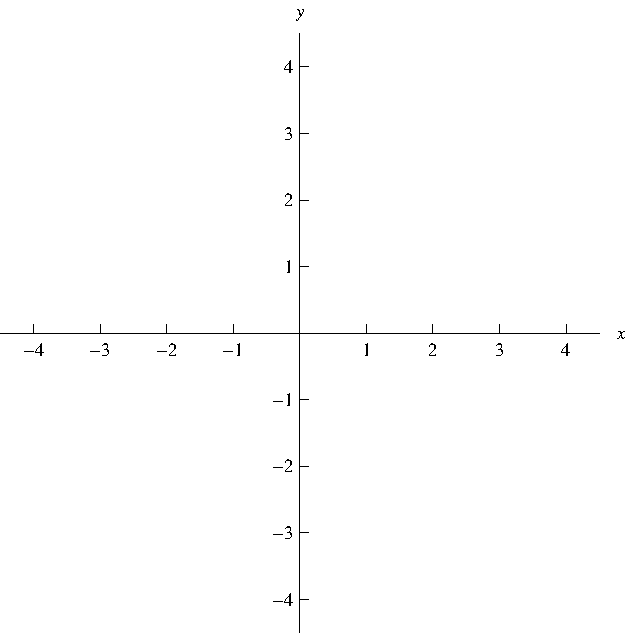
\includegraphics[height=6cm]{parametric-curves/pictures/11-01-ex1a.pdf}%
%}%
%\only<handout:0| 3-4>{%
%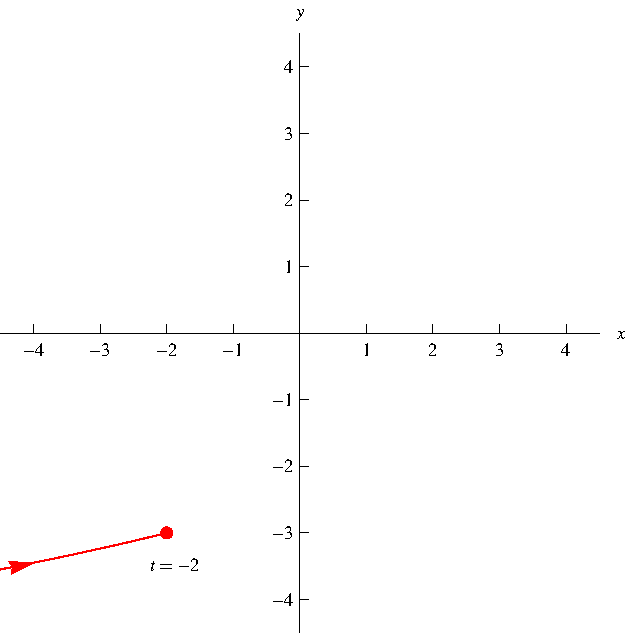
\includegraphics[height=6cm]{parametric-curves/pictures/11-01-ex1b.pdf}%
%}%
%\only<handout:0| 5-6>{%
%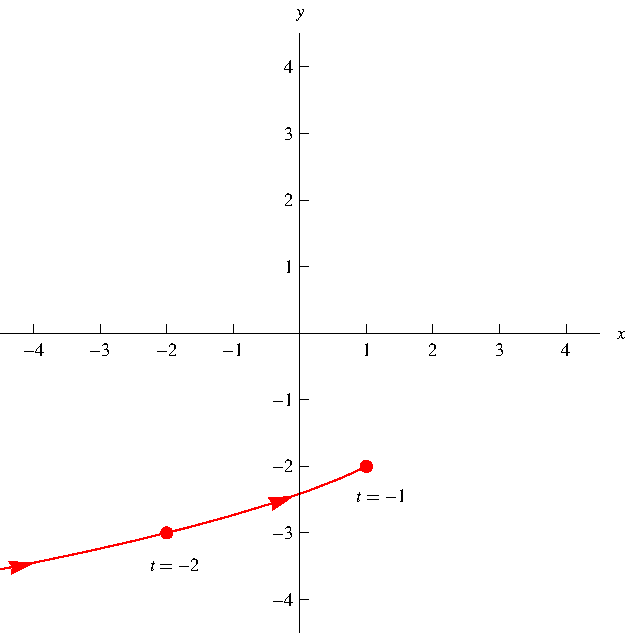
\includegraphics[height=6cm]{parametric-curves/pictures/11-01-ex1c.pdf}%
%}%
%\only<handout:0| 7-8>{%
%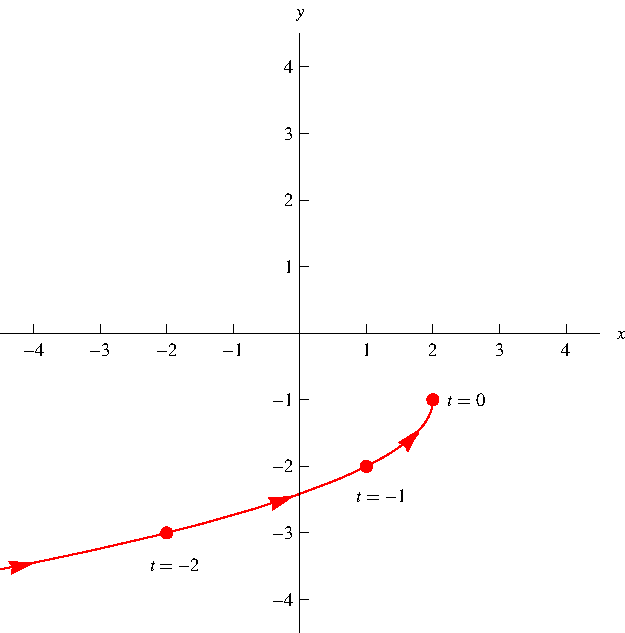
\includegraphics[height=6cm]{parametric-curves/pictures/11-01-ex1d.pdf}%
%}%
%\only<handout:0| 9-10>{%
%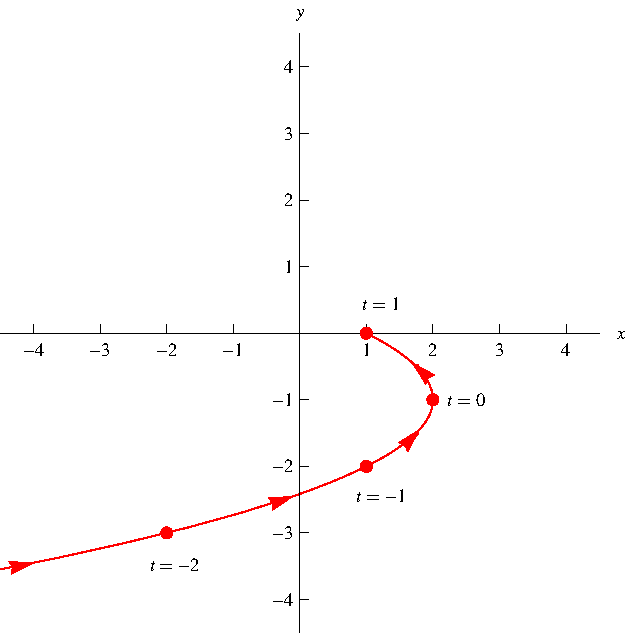
\includegraphics[height=6cm]{parametric-curves/pictures/11-01-ex1e.pdf}%
%}%
%\only<handout:0| 11>{%
%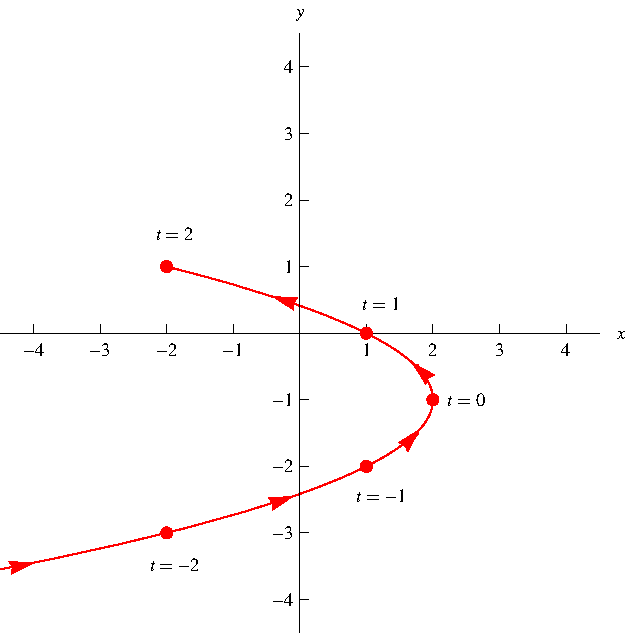
\includegraphics[height=6cm]{parametric-curves/pictures/11-01-ex1f.pdf}%
%}%
%\only<12->{%
%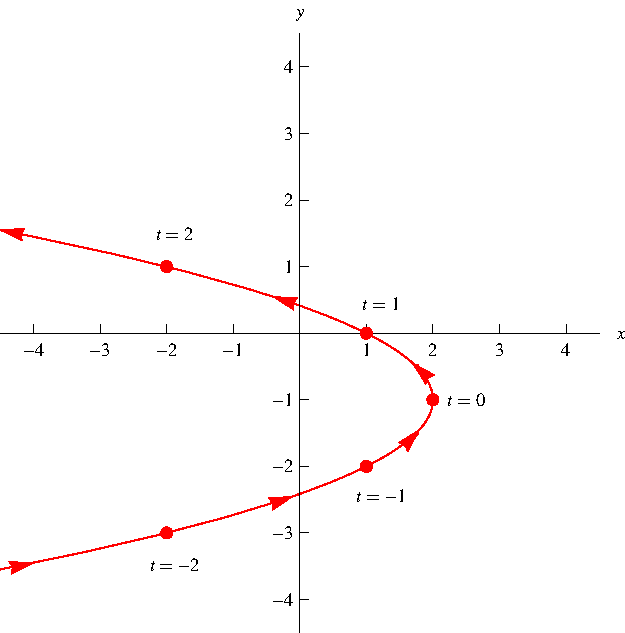
\includegraphics[height=6cm]{parametric-curves/pictures/11-01-ex1g.pdf}%
%}%
\column{.5\textwidth}
\hfil \hfil
$
\begin{array}{|r|r|r|}
\hline
\alert<2,4,6,8,10>{ t} & x & y\\
\hline
\alert<handout:0| 2-3>{-2} &%
\alert<handout:0| 2-3>{\uncover<3->{-2}} &%
\alert<handout:0| 2-3>{\uncover<3->{-3}} \\%
\alert<handout:0| 4-5>{-1} &%
\alert<handout:0| 4-5>{\uncover<5->{1}} &%
\alert<handout:0| 4-5>{\uncover<5->{-2}} \\%
\alert<handout:0| 6-7>{0} &%
\alert<handout:0| 6-7>{\uncover<7->{2}} &%
\alert<handout:0| 6-7>{\uncover<7->{-1}} \\%
\alert<handout:0| 8-9>{1} &%
\alert<handout:0| 8-9>{\uncover<9->{1}} &%
\alert<handout:0| 8-9>{\uncover<9->{0}} \\%
\alert<handout:0| 10-11>{2} &%
\alert<handout:0| 10-11>{\uncover<11->{-2}} &%
\alert<handout:0| 10-11>{\uncover<11->{1}} \\%
\hline
\end{array}
$
\hfil

\uncover<14->{%
\noindent Eliminate $t$: from second equation we have $\alert<handout:0| 14,16>{t = y + 1}$ \uncover<15->{%
and therefore:}  %
}%
$\begin{array}{rcl}
\uncover<15->{%
\alert<handout:0| 15,18>{x}%
}%
&\uncover<15->{\alert<handout:0| 15>{ =}}&%
\uncover<15->{%
\alert<handout:0| 15>{ -\alert<handout:0| 16>{t}^2 + 2}%
}\\%
& \uncover<16->{ = }&%
\uncover<16->{%
 -(\alert<handout:0| 16>{y+1})^2 + 2
}\\%
& \uncover<17->{\alert<handout:0| 18>{ = }}&%
\uncover<17->{%
\alert<handout:0| 18>{-y^2 - 2y + 1}
}%
\end{array}
$

\uncover<18->{Thus our curve image is a parabola, as expected.}
\end{columns}
\end{example}
\end{frame}

\begin{frame}
\begin{columns}[c]
\column{.5\textwidth}
%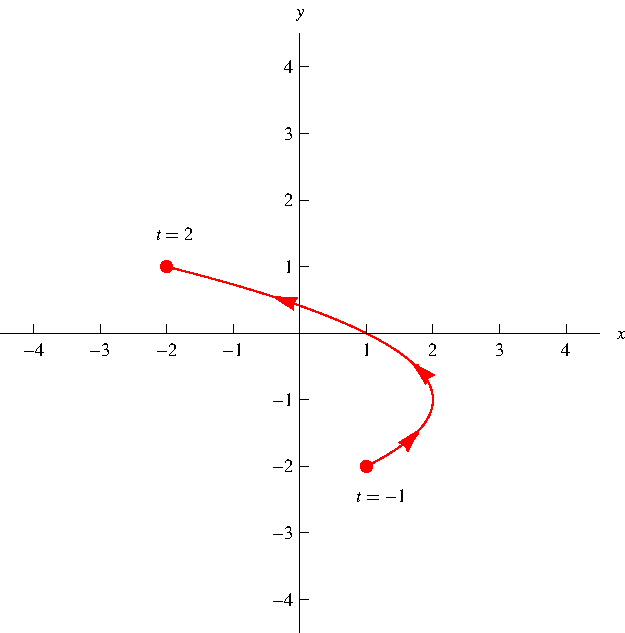
\includegraphics[height=6cm]{parametric-curves/pictures/11-01-ex1chopped.pdf}%
\psset{xunit=0.8cm, yunit=0.8cm}
\begin{pspicture}(-1.000000, -5)(1.500000,5) 
\psframe*[linecolor=white](-7.000000,-7)(5,5) 
\tiny 
\psaxes[arrows=<->](0,0)(-4.3, -4)(3, 2)
\psLabels{3}{2}
%Calculator input: plotCurve{}(- t^{2}+2, t-1, -2, 2)

\uncover<1-3>{ 
\parametricplot[linecolor=\psColorGraph, arrows=->, plotpoints=150]{ -2.5 }{-1.25}{2 t 2 exp -1 mul add -1 t add }
\parametricplot[linecolor=\psColorGraph, arrows=->, plotpoints=150]{ -1.25 }{0}{2 t 2 exp -1 mul add -1 t add }
\parametricplot[linecolor=\psColorGraph, arrows=->, plotpoints=150]{ 0 }{1.25}{2 t 2 exp -1 mul add -1 t add }
\parametricplot[linecolor=\psColorGraph, plotpoints=150]{ 1.25 }{2.5}{2 t 2 exp -1 mul add -1 t add }
}
\uncover<4->{ 
\parametricplot[linecolor=\psColorGraph, plotpoints=150]{ -1 }{0}{2 t 2 exp -1 mul add -1 t add }
\parametricplot[linecolor=\psColorGraph, arrows=->, plotpoints=150]{ 0 }{1}{2 t 2 exp -1 mul add -1 t add }
\parametricplot[linecolor=\psColorGraph, plotpoints=150]{ 1 }{2}{2 t 2 exp -1 mul add -1 t add }
}
\uncover<5->{
\psFullDot{-2}{1}
\psFullDot{1}{-2}
}
\end{pspicture}
\[
\left|\begin{array}{rcl}
\alert<handout:0| 15>{x } & \alert<handout:0| 15>{=} & \alert<handout:0| 15>{ -{\alert<2, 4,6,8,10> {t}}^2 + 2}\\
\alert<14>{y}&\alert<14>{=}&\alert<14>{ \alert<2, 4,6,8,10> {t}-1}
\end{array}\right.\uncover<4->{,
 -1 \leq t \leq 2}
\]
\column{.5\textwidth}
\begin{itemize}
\item<1->  There was no restriction placed on $t$ in the last example. 
\item<2->  In such a case we assume $t\in (-\infty,\infty)$, i.e., $t$ runs over all real numbers.
\item<3->  In general we are expected to specify the interval in which $t$ lies.
\item<4->  For example, if we restrict the previous example to $t\in [-1,2]$, we get the part of the parabola that begins at $(1,-2)$ and ends at $(-2,1)$.
\item<5->  We say that  $(1,-2)$ is the initial point and $(-2,1)$ is the terminal point of the curve.
\end{itemize}
\end{columns}
\end{frame}
% end module eliminate-parameter-ex
